% 第3章第6节：最小费用流（问题；最优性条件；网络单纯形法；统一表示；结果检验）。

\section{最小费用流}
\label{sec:graph-min-cost-flow}

第~\ref{sec:graph-max-flow}节只问能送多少。实际调运中，各处的产量与需求事先给定，各条线路运价不同，要比较的是满足供需的方案中哪个总费用最低。本节把容量、供需和单位费用放进同一个模型，并说明前面的输送与配对问题都是它的特例。

对方案的任何改动，都可以看成把一部分货物从一条线路挪到另一条线路，也就是沿一个环改道。有省钱的环，当前方案就不是最优；没有，就是最优。\term{网络单纯形法}（network simplex method，亦称网络单形法）把方案记在一棵生成树上，每次只沿一个环改道。它是线性规划单纯形法在网络上的特例，这里只用树、环和守恒式建立它，一般理论留到后续优化部分。

\subsection{最小费用流问题}
\label{sec:graph-opt-mcf-problem}

设想几个仓库经中转站向几家商店供货：库存要全部运出，需求要恰好满足；每条线路有运量上限，有些按合同还有最低运量，每运一单位付相应的运价。把各处看成顶点、线路看成有向弧，就得到下面的问题。为了把字母$c$留给费用，本节把容量改记为上界$u_{i,j}$，弧写作$(i,j)$或$i\to j$。

\begin{definition}[最小费用流问题]
\label{def:graph-opt-min-cost-flow}
设$\mathcal G=(V,E)$是有限有向图，每个顶点$i$有供需量$b_i\in\mathbb R$，每条弧$(i,j)\in E$有有限的下界$\ell_{i,j}$、上界$u_{i,j}$（$\ell_{i,j}\leq u_{i,j}$）与单位费用$c_{i,j}\in\mathbb R$。给每条弧赋一个流量$x_{i,j}$，若向量$\bm x$满足
\begin{equation}
\begin{gathered}
  \sum_{j:\,(i,j)\in E}x_{i,j}-\sum_{j:\,(j,i)\in E}x_{j,i}=b_i\quad(i\in V),\\
  \ell_{i,j}\leq x_{i,j}\leq u_{i,j}\quad((i,j)\in E),
\end{gathered}
  \label{eq:graph-opt-mcf-constraints}
\end{equation}
则称$\bm x$为可行流。\term{最小费用流}（minimum-cost flow）问题是在全部可行流中最小化总费用$\sum_{(i,j)\in E}c_{i,j}x_{i,j}$。
\end{definition}

守恒式左边是顶点$i$的净流出，所以$b_i>0$表示$i$是供给点，要净送出$b_i$单位；$b_i<0$表示需求点，要净收进$-b_i$单位；$b_i=0$的顶点只做中转。把全部守恒式相加，每条弧的流量正负各计一次，左边为零，所以$\sum_{i\in V}b_i=0$是可行流存在的必要条件。它不充分：平衡的供需不保证有路可走、容量够用。图~\ref{fig:graph-opt-mcf-network}的网络中，若把$s\to a$与$s\to t$的容量都改成$1$，从$s$出发的总容量只有$2$，供需虽然平衡，问题却没有可行流。

\begin{figure}[!htb]
  \centering
  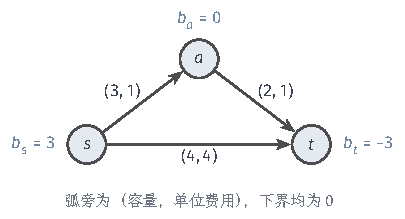
\includegraphics[width=68.527mm]{figures/01-basic-mathematics/04-graphs/tikz/c3-mcf-network/figure.pdf}
  \caption{三点最小费用流算例。$s$供给$3$单位，$t$需求$3$单位，$a$只做中转；弧旁括号依次为容量与单位费用，下界均为$0$。绕行$s\to a\to t$的单位费用为$2$，低于直达弧的$4$，但绕行量受$a\to t$的容量$2$限制。}
  \label{fig:graph-opt-mcf-network}
\end{figure}

按弧序$s\to a$、$a\to t$、$s\to t$把流量写成向量：$3$单位全走直达弧是$(0,0,3)$，费用$3\times4=12$；让$2$单位绕行、$1$单位直达是$(2,2,1)$，费用$2\times(1+1)+1\times4=8$。后面将证明$8$就是最小费用。

正下界（如合同规定的最低运量）的处理办法是先把下界部分“预先送出”，再对剩余部分求解。令$x_{i,j}=\ell_{i,j}+y_{i,j}$，新变量满足$0\leq y_{i,j}\leq u_{i,j}-\ell_{i,j}$。预先送出的下界流量已经使顶点$i$净流出$\sum_j\ell_{i,j}-\sum_j\ell_{j,i}$，所以$\bm y$应满足的剩余供需为
\[
  b'_i=b_i-\sum_{j:\,(i,j)\in E}\ell_{i,j}+\sum_{j:\,(j,i)\in E}\ell_{j,i}.
\]
目标变为$\sum c_{i,j}y_{i,j}+\bm c^{\top}\bm\ell$，后一项是常数。两个问题的可行解与最优解通过$\bm x=\bm\ell+\bm y$一一对应。图~\ref{fig:graph-opt-mcf-lower-bound}把三点网络中$s\to t$的下界改为$1$：这条弧的容量从$4$变为$3$，$s$的剩余供给从$3$降为$2$，$t$的剩余需求从$3$降为$2$，目标另加常数$c_{s,t}\ell_{s,t}=4$。只改容量而不改供需，下界那一单位就被重复计算。新问题的最优解是$\bm y=(2,2,0)$，费用$4$；加回下界与常数，得到原问题的最优流$\bm x=(2,2,1)$与费用$8$。上下界相等的固定弧平移后容量为零，可以先删去，只保留它对供需和常数的贡献。以下除非特别说明，都假定下界已平移为零、固定弧已删去。

\begin{figure}[!htb]
  \centering
  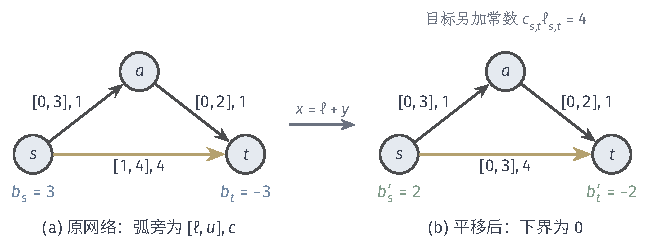
\includegraphics[width=109.767mm]{figures/01-basic-mathematics/04-graphs/tikz/c3-mcf-lower-bound-shift/figure.pdf}
  \caption{下界平移。(a)中黄色弧$s\to t$的流量须在$[1,4]$内，弧旁依次为流量区间与单位费用。(b)令$x=\ell+y$后，该弧的区间变为$[0,3]$，$s$与$t$的供需同时各减少$1$单位（绿色），目标另加常数$4$。}
  \label{fig:graph-opt-mcf-lower-bound}
\end{figure}

从源点$s$向汇点$t$输送固定量$F$时，令$b_s=F$、$b_t=-F$，其余$b_i=0$。全部$b_i=0$时的可行流称为\term{循环流}（circulation）；第~\ref{sec:graph-opt-mcf-unified}小节会用它表达最大流。先尽量多送、再在全部最大流中挑费用最低的，称为\term{最小费用最大流}（minimum-cost maximum flow）：先用第~\ref{sec:graph-max-flow}节的方法求出最大流值$v^\star$，再取$F=v^\star$。

在有限上下界下，可行流集合是$\mathbb R^{a}$中的闭有界集（$a=|E|$），总费用是线性函数，由极值定理~\ref{thm:multivariable-extreme-value}，只要可行流存在，最小费用一定能取到；可行性由后文网络单纯形法的第一阶段判断。若允许无穷容量，可无限推送的负费用环使费用没有下界；本节主线只讨论有限容量，无穷容量放在第~\ref{sec:graph-opt-ns-improvements}小节。

\subsection{费用残量网络与最优性条件}
\label{sec:graph-opt-mcf-optimality}

判断最优不能逐一比较全部可行流。这里沿用第~\ref{sec:graph-opt-residual-network}小节的残量网络描述流量还能怎样改，只是每条残量弧多带一个费用。

给定可行流$\bm x$。对每条原弧$(i,j)$，若$x_{i,j}<u_{i,j}$，建立正向残量弧$i\to j$，剩余容量$u_{i,j}-x_{i,j}$，费用$c_{i,j}$；若$x_{i,j}>\ell_{i,j}$，建立反向残量弧$j\to i$，剩余容量$x_{i,j}-\ell_{i,j}$，费用$-c_{i,j}$，表示撤回一单位省下$c_{i,j}$。原网络同时有$i\to j$与$j\to i$两条弧时，各自的残量弧要记住来自哪条原弧，不能合并。

改道在残量网络中就是一个环。图~\ref{fig:graph-opt-mcf-residual-cycle}从全走直达的流$(0,0,3)$出发：把一单位改走中转，要在$s\to a$、$a\to t$各加一单位，并从直达弧撤回一单位，三步首尾相接成残量环$s\to a\to t\to s$，费用$1+1-4=-2$。逐点看，$s$、$a$、$t$各自少走一条弧、多走一条弧，净流出不变。逐边看，$s\to a$还能加$3$，$a\to t$还能加$2$，直达弧还能撤回$3$，所以最多改道$\min\{3,2,3\}=2$单位，费用从$12$降为$8$。

\begin{figure}[!htb]
  \centering
  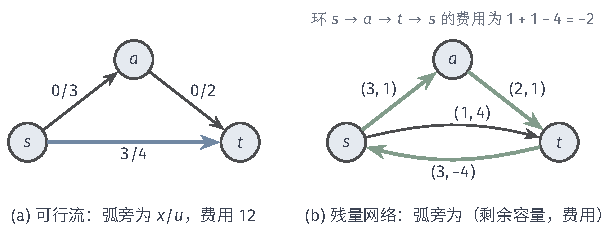
\includegraphics[width=103.579mm]{figures/01-basic-mathematics/04-graphs/tikz/c3-mcf-residual-cycle/figure.pdf}
  \caption{残量网络中的负费用环。(a)全部$3$单位走直达弧的可行流，弧旁为流量与容量。(b)它的残量网络，弧旁为剩余容量与费用；直达弧产生可追加$1$单位的正向弧和可撤回$3$单位、费用$-4$的反向弧$t\to s$。绿色环费用$-2$，推送$2$单位使费用降$4$。}
  \label{fig:graph-opt-mcf-residual-cycle}
\end{figure}

一般地，沿残量网络中的有向环$C$推送$\theta>0$单位，是指正向残量弧对应的原弧流量加$\theta$，反向残量弧对应的原弧流量减$\theta$。环上每个顶点恰有一条环弧进入、一条离开，净流出不变；$\theta$不超过环上的最小剩余容量时，上下界仍然满足。费用改变$\theta\,c(C)$，其中$c(C)$是环上残量费用之和。所以有$c(C)<0$的环时当前流不是最优。反过来也成立，关键是任何可行流与当前流之差都能拆成残量环的叠加。

\begin{theorem}[负费用环判据]
\label{thm:graph-opt-negative-cycle}
可行流$\bm x$是最小费用流，当且仅当它的残量网络中不存在费用为负的有向环。
\end{theorem}

\begin{proof}
必要性已由上面的推送论证给出，下证充分性。任取可行流$\bm x'$，令$\bm d=\bm x'-\bm x$。两个流满足同一组供需，所以$\bm d$在每个顶点的净流出为零。逐条考察原弧$(i,j)$：若$d_{i,j}>0$，则$x_{i,j}<x'_{i,j}\leq u_{i,j}$，正向残量弧存在且剩余容量至少为$d_{i,j}$，在它上面放$d_{i,j}$；若$d_{i,j}<0$，则$x_{i,j}>x'_{i,j}\geq\ell_{i,j}$，反向残量弧存在，在它上面放$-d_{i,j}$。这样得到残量弧上的一组非负数$\bm g$，它在每个顶点流入等于流出，按残量费用加权的总和等于$\bm c^{\top}\bm x'-\bm c^{\top}\bm x$。

若$\bm g\neq\bm 0$，从任一取正值的残量弧出发，沿正值弧前进：每到达一个顶点，它的流入为正，必有一条正值出弧可走。顶点有限，前进中必然回到某个走过的顶点，截出一个有向环$C_1$。令$\lambda_1>0$为$\bm g$在$C_1$上的最小值，从环上各弧减去$\lambda_1$，剩余部分仍非负且守恒，而取正值的弧至少少了一条。重复有限次，得到
\[
  \bm c^{\top}\bm x'-\bm c^{\top}\bm x=\sum_k\lambda_k\,c(C_k),\qquad\lambda_k>0.
\]
每个$C_k$都由残量弧组成。残量网络中没有负费用环时，右边每项非负，$\bm x'$不比$\bm x$便宜。
\end{proof}

判据不是完整的算法，也不断言最优流唯一；而且环的个数可能随规模指数增长。为了改为逐弧检查，给每个顶点$i$配一个实数$\pi_i$，称为\term{节点势}（node potential），并定义弧$(i,j)$的\term{约化费用}（reduced cost）
\begin{equation}
  \bar c_{i,j}=c_{i,j}-\pi_i+\pi_j.
  \label{eq:graph-opt-reduced-cost}
\end{equation}
残量弧使用同一公式：反向残量弧$j\to i$的费用为$-c_{i,j}$，约化费用为$-c_{i,j}-\pi_j+\pi_i=-\bar c_{i,j}$。沿有向环相加时，每个顶点的势在出弧上以$-\pi$、在入弧上以$+\pi$各出现一次，相消，所以环的约化费用等于原费用。因此，若能找到一组势，使所有残量弧的约化费用都非负，残量网络就没有负费用环。

反过来，残量网络没有负费用环时，这样的势一定存在。加入虚拟顶点$r$，向每个顶点连一条零费用弧；新图的环不经过$r$，仍无负环。记$d_i$为$r$到$i$的最短路径费用，绕环不会更便宜，只需比较有限条简单路径，所以$d_i$有限。对残量弧$i\to j$及其费用$c'$，到$i$的最短路径接上这条弧是一条到$j$的行走，去掉其中的环不增加费用，所以$d_j\leq d_i+c'$。取$\pi_i=-d_i$，即得$c'-\pi_i+\pi_j=c'+d_i-d_j\geq0$。实际可用第~\ref{sec:graph-opt-bellman-ford}小节的Bellman--Ford算法求$d_i$，它报告负环时就找到了可推送的负费用环。

势可以理解为各顶点上货物的“边际运费”。把$\pi_i$看成从$i$再送一单位到需求点$t$的最低费用（$\pi_t=0$），允许借助残量弧撤回已有流量。图~\ref{fig:graph-opt-mcf-potentials}以流$(2,2,1)$为例：从$s$再送一单位，绕行已被$a\to t$卡住，只能直达，$\pi_s=4$；从$a$再送一单位，最便宜的是让一单位原本经$a$绕行的货改走直达，$a$处这单位顶替它前往$t$，省$1$付$4$，$\pi_a=3$。这正是由最短距离构造的势。

\begin{figure*}[!htb]
  \centering
  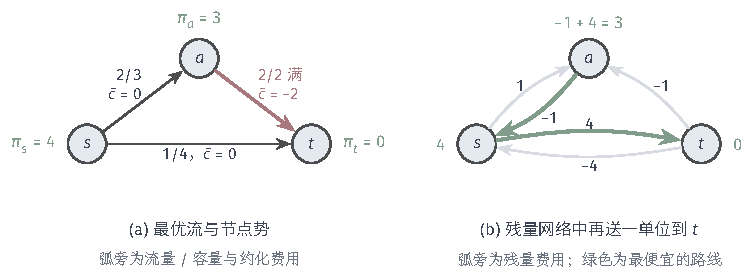
\includegraphics[width=127.593mm]{figures/01-basic-mathematics/04-graphs/tikz/c3-mcf-potentials/figure.pdf}
  \caption{节点势的直观含义。(a)流$(2,2,1)$与势$(4,3,0)$；界内弧约化费用为零，满载弧$a\to t$为$-2$（红色）。(b)残量网络，弧旁为残量费用；绿色为从各顶点再送一单位到$t$的最便宜路线，费用$4$与$3$即$\pi_s,\pi_a$。}
  \label{fig:graph-opt-mcf-potentials}
\end{figure*}

按这种理解，约化费用$\bar c_{i,j}=c_{i,j}+\pi_j-\pi_i$比较两种送货方式：经弧$(i,j)$送出一单位，付$c_{i,j}$再付$\pi_j$；或按$i$现行的边际方式送出，付$\pi_i$。$\bar c_{i,j}<0$表示这条弧更便宜，应当多用；$\bar c_{i,j}>0$表示更贵，应当少用。最优流中能加量的弧不能更便宜，能减量的弧不能更贵。“全部残量弧约化费用非负”于是逐弧翻译为：弧在下界时只有正向残量弧，要求$\bar c_{i,j}\geq0$；在上界时只有反向残量弧，要求$\bar c_{i,j}\leq0$；严格在两界之间时两条都存在，要求$\bar c_{i,j}=0$。

\begin{theorem}[节点势最优性证书]
\label{thm:graph-opt-potential-certificate}
设固定弧已删去，$\bm x$是可行流，$\bm\pi$是一组节点势。若对每条弧$(i,j)$都有
\begin{equation}
  \bar c_{i,j}\ \begin{cases}
    \geq0, & x_{i,j}=\ell_{i,j},\\
    \leq0, & x_{i,j}=u_{i,j},\\
    =0, & \ell_{i,j}<x_{i,j}<u_{i,j},
  \end{cases}
  \label{eq:graph-opt-mcf-certificate}
\end{equation}
则$\bm x$是最小费用流。
\end{theorem}

\begin{proof}
任取可行流$\bm x'$。把$c_{i,j}=\bar c_{i,j}+\pi_i-\pi_j$代入费用差，
\[
  \bm c^{\top}(\bm x'-\bm x)=\sum_{(i,j)\in E}\bar c_{i,j}(x'_{i,j}-x_{i,j})+\sum_{(i,j)\in E}(\pi_i-\pi_j)(x'_{i,j}-x_{i,j}).
\]
第二个和按顶点归组，等于对每个$i$把$\pi_i$乘以顶点$i$在$\bm x'$与$\bm x$下净流出之差再求和；两个流满足同一组供需，这些差全为零。第一个和逐项非负：若$x_{i,j}=\ell_{i,j}$，则$x'_{i,j}-x_{i,j}\geq0$且$\bar c_{i,j}\geq0$；若$x_{i,j}=u_{i,j}$，则$x'_{i,j}-x_{i,j}\leq0$且$\bar c_{i,j}\leq0$；其余情形$\bar c_{i,j}=0$。所以$\bm c^{\top}\bm x'\geq\bm c^{\top}\bm x$。
\end{proof}

删去固定弧是为了避免$\ell_{i,j}=u_{i,j}$时前两个条件同时出现。这组条件在线性规划中称为互补松弛条件。流量与势合起来构成证书：核对可行性和每条弧上的一个符号，就能确认最优，不必相信求解过程。在三点网络中取流$(2,2,1)$与势$(4,3,0)$，界内的两条弧$s\to a$、$s\to t$的约化费用都是零，上界弧$a\to t$的约化费用为$-2\leq0$，所以费用$8$最小。

\subsection{网络单纯形法}
\label{sec:graph-opt-network-simplex}

本算法用可行树基记录流量，用非树弧的约化费用寻找改善方向，再沿基本环调整。

\subsubsection{主要思想}

前一小节把三点网络的改道写成了负费用环$s\to a\to t\to s$：每改道一单位省$2$，最多改$2$单位，费用$12\to8$。负环指明了改进方向，剩下的问题是有组织地找到它们：记录当前流的方式应使候选的环容易列出，环的费用和改道量容易算出。

办法是把流记在一棵树上。规定$s\to a$的流量固定为$0$，只让$s\to t$与$a\to t$待定：中转点$a$没有外部供需，所以$a\to t=0$；$t$要收的$3$单位只能来自$s\to t$，所以$s\to t=3$。固定一部分弧后，其余流量顺着树由守恒式算出。一般地，忽略方向后构成生成树的弧集记为$T$，称为树弧；其余弧的流量固定在下界或上界，分别组成$L$与$U$。三元组$(T,L,U)$称为一个\term{树基}（spanning tree basis）。叶子只关联一条树弧，它的守恒式中其余各项已知，于是解出这条树弧的流量；删去叶子再重复，就求出全部树弧流量。若它们都在上下界内，称$(T,L,U)$为可行树基。

把$s\to a$加进树，恰好多出一个环，正是上面的改道环。一般地，非树弧与树上连接其两端的唯一路径合成的环称为\term{基本环}（fundamental cycle）。沿这个环推送$2$单位后，$a\to t$到达上界，它退出树、进入$U$，$s\to a$进入树。这一步称为换基：它同时更新了表示当前流的树，使新流$(2,2,1)$仍由新树确定。

只在树形方案中寻找，不会错过最优解。若严格位于两界之间的弧含有一个环，沿环的两个方向都能推送少量流量，两方向单位费用变化互为相反数，至少一个方向不增加费用；沿它推到某条弧碰界，环就被打断。反复这样做，界内弧不再含环，补上一些在界上的弧即成生成树。图~\ref{fig:graph-opt-ns-why-tree}中，流$(1,1,2)$的三条弧都在界内而成环，推送$1$单位后$a\to t$满载，得到$(2,2,1)$，环被打断。树形方案只有有限多个。

\begin{figure*}[!htb]
  \centering
  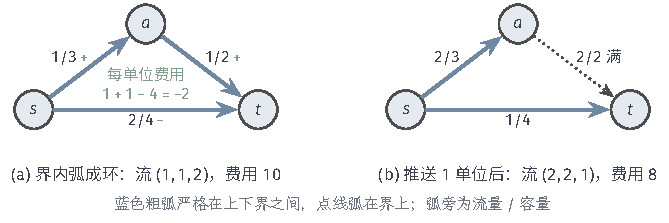
\includegraphics[width=113.249mm]{figures/01-basic-mathematics/04-graphs/tikz/c3-ns-why-tree/figure.pdf}
  \caption{打断界内弧的环。(a)流$(1,1,2)$的三条弧都在界内，按绿色符号沿环推送，每单位费用变化$-2$。(b)推送$1$单位后$a\to t$到上界，界内弧不再成环，费用由$10$降为$8$。}
  \label{fig:graph-opt-ns-why-tree}
\end{figure*}

同一棵树还给出节点势。令$\pi_t=0$，要求两条树弧约化费用为零，得$\pi_s=4$、$\pi_a=1$；候选弧$s\to a$的约化费用$1-4+1=-2$恰是每改道一单位的费用变化。这不是巧合：把基本环上每个$c$换成$\bar c+\pi_i-\pi_j$，势相消，树弧约化费用为零，只剩非树弧自己的约化费用。所以定价，即检查非树弧约化费用的符号，就是逐个评估全部基本环。树上的路径可能逆着原弧方向走，$\pi_i-\pi_j$是沿树从$i$到$j$的有符号费用，顺弧计正、逆弧计负；它一般不是全图中的最短距离，前一小节的“边际运费”是针对最优流说的。

概括起来，网络单纯形法只做三件事：只在树形方案中寻找；用一棵树同时决定流和势；每次找一条约化费用符号不对的非树弧，沿它的基本环改道，改到某条弧碰界为止，再让这条弧离开树。图~\ref{fig:graph-opt-ns-loop}画出了这个循环，系统的讲述可参考Bertsekas的网络优化教材\scite{math-graph-bertsekas1998network}。

\begin{figure*}[!htb]
  \centering
  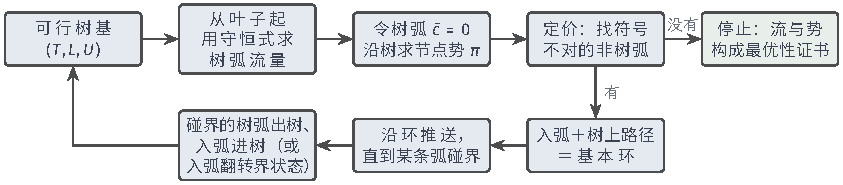
\includegraphics[width=142.762mm]{figures/01-basic-mathematics/04-graphs/tikz/c3-ns-loop/figure.pdf}
  \caption{网络单纯形法的一轮。定价后若无符号不对的非树弧就停止，否则沿基本环推送到某弧碰界：碰界的树弧出树、入弧进树，或入弧自身翻转界状态。}
  \label{fig:graph-opt-ns-loop}
\end{figure*}

\subsubsection{算法流程}

\paragraph{算法状态}
手算用到的记录——每条弧送多少、哪些弧成树、其余弧停在哪个界、各点势多少——列在表~\ref{tab:graph-opt-ns-state}中，并以$t$为根记下每个顶点的父顶点、父边与深度。父顶点和父边用于沿树找路，深度帮助入弧两端回溯到公共祖先。

\begin{table}[!htb]
  \centering\small
  \caption{三点网络在树$T=\{s\to t,a\to t\}$下的状态，根为$t$。左表为弧记录，右表为顶点记录。}
  \label{tab:graph-opt-ns-state}
  \begin{tabular}{@{}lcccc@{}}
    \toprule
    弧 & 流量 & 界 & 费用 & 状态 \\
    \midrule
    $s\to a$ & $0$ & $[0,3]$ & $1$ & $L$ \\
    $a\to t$ & $0$ & $[0,2]$ & $1$ & $T$ \\
    $s\to t$ & $3$ & $[0,4]$ & $4$ & $T$ \\
    \bottomrule
  \end{tabular}\quad
  \begin{tabular}{@{}lcccc@{}}
    \toprule
    顶点 & 势 & 父顶点 & 父边 & 深度 \\
    \midrule
    $s$ & $4$ & $t$ & $s\to t$ & $1$ \\
    $a$ & $1$ & $t$ & $a\to t$ & $1$ \\
    $t$ & $0$ & — & — & $0$ \\
    \bottomrule
  \end{tabular}
\end{table}

平移下界、删去固定弧后的网络及其邻接结构在开始前构造，运行中不变，不算状态。算法维护以下状态：
\begin{itemize}
  \item 树基$(T,L,U)$：初值为第一阶段的星形树基，第二阶段开始时换成清理人工结构后得到的树基；
  \item 各弧流量$x_{i,j}$：初值由初始树基逐叶解出，连同防循环规则所需的扰动系数一起存储；
  \item 节点势$\pi_i$：根的势为零，其余由树弧约化费用为零解出；
  \item 树的记录$\mathrm{parent}(i)$、$\mathrm{parent\_edge}(i)$、$\mathrm{depth}(i)$：取一个顶点为根，初值由一次树遍历得到。
\end{itemize}
树弧的流量允许恰好在界上：一条弧是否属于$T$取决于它在树中的位置，而不是流量是否在界内。所以同一个流可能对应不同的树基，后面的退化现象正来自这种区别。

势沿树求解：根的势为零，沿树弧方向从已知的$\pi_i$走到$j$时取$\pi_j=\pi_i-c_{i,j}$，逆着树弧方向从已知的$\pi_j$走到$i$时取$\pi_i=\pi_j+c_{i,j}$。换一个根只让全部势同加一个常数，约化费用不变。生成树要求底层无向图连通。消去固定弧后若原图不连通，就在各弱连通分量中分别处理：每个分量内的剩余供需之和必须为零，否则问题不可行；孤立顶点没有任何弧，它的供需必须为零。

\paragraph{初始化与第一阶段}
随手选的树未必可行：在三点网络中取$T=\{s\to a,a\to t\}$、令$s\to t$取下界，叶子$s$与$t$迫使$x_{s,a}=x_{a,t}=3$，超过$a\to t$的容量$2$。办法是暂时“借用”虚拟线路：加一个只供记账的人工中转点$r$，$s$把$3$单位送进$r$，$r$再送$3$单位给$t$，$a$用零流量的人工弧$a\to r$接入。账目先平衡了，但这不代表原网络可行。

一般地，在下界已平移为零的网络中令全部原弧流量为零，供给点连人工弧$i\to r$、流量$b_i$，需求点连人工弧$r\to i$、流量$-b_i$，零供需点连人工弧$i\to r$、流量$0$；人工弧容量取总供给$\sum_{b_i>0}b_i$。人工弧构成以$r$为中心的星形生成树，是显式的可行树基。

借用的线路要尽量还回去。第一阶段令人工弧每单位记费用$1$、原弧记$0$，目标就是人工流总量，用下面同一套选弧、环调整与防循环操作求解。最优值为零即原问题可行，为正即不可行（定理~\ref{thm:graph-opt-network-simplex}）。在三点网络中，星形树为$s\to r$、$r\to t$、$a\to r$，流量$3,3,0$，人工流总量$6$。以$r$为根，势为$(\pi_s,\pi_a,\pi_t)=(1,1,-1)$，先选约化费用为$-2$的$s\to t$入树，沿环$s\to t\to r\to s$推送$3$单位，$s\to r$与$r\to t$同时降为零，防循环规则选$s\to r$出树；再选$a\to t$入树，环上的$r\to t$与$a\to r$都已为零，步长为零，规则选$a\to r$出树。此时人工流为零，见图~\ref{fig:graph-opt-ns-artificial-start}。

\begin{figure*}[!htb]
  \centering
  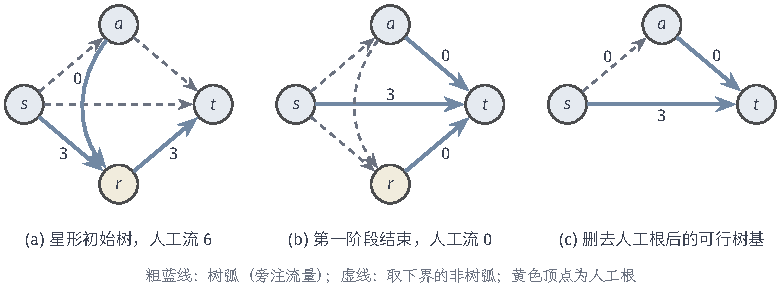
\includegraphics[width=132.186mm]{figures/01-basic-mathematics/04-graphs/tikz/c3-ns-artificial-start/figure.pdf}
  \caption{两阶段法的第一阶段。(a)人工根$r$（黄色）与人工弧构成星形可行树，人工流为$6$。(b)两次换基后人工流为零，$s\to t$承担$3$单位，空载的$r\to t$仍在树中。(c)删去人工结构，剩下的树弧构成原网络的生成树，作为第二阶段的初始树基。}
  \label{fig:graph-opt-ns-artificial-start}
\end{figure*}

人工流归零后删去人工根和全部人工弧。原来的树弧去掉人工弧后留下一个森林；在原图的每个弱连通分量内，用连接不同森林分量的原非树弧把它补成生成树。补入的弧保持原流量，作为树弧恰在界上是允许的。随后恢复原费用、重新计算势，并从所得的普通可行树基重新设置防循环数据，进入第二阶段。三点网络中删去$r$后，$s\to t$与$a\to t$已经构成生成树，$s\to a$在下界。

\paragraph{选入弧与沿环调整}
每一轮按以下步骤进行：
\begin{itemize}
  \item 定价：用当前势计算非树弧的约化费用。$L$中$\bar c_{i,j}<0$的弧应沿正向增加流量，$U$中$\bar c_{i,j}>0$的弧应沿反向减少流量；从这些违反条件的弧中选一条作为入弧。
  \item 找环：从入弧两端沿父指针上溯，深度大的一端先走，深度相同后一起走，相遇处是最近公共祖先；两段路径与入弧合成基本环。按入弧的调整方向给环定向，顺着定向经过的弧增加流量，逆着定向经过的弧减少流量。
  \item 求步长：增加的弧计算$u-x$，减少的弧计算$x-\ell$，入弧自身也参加比较，取最小值作为步长$\theta$。达到最小值的弧称为阻塞弧，可能不止一条，按防循环规则从中选出一条作为出弧。
  \item 更新流量：增加的弧加$\theta$、减少的弧减$\theta$，费用改变$\theta$乘以入弧在调整方向上的约化费用，$\theta>0$时严格下降。
  \item 更新树基：出弧是树弧时，它离开树，按到达的是下界还是上界归入$L$或$U$，入弧加入$T$，再更新父顶点、深度与势。出弧是入弧自身时，入弧在$L$与$U$之间翻转，树和势都不变。
\end{itemize}

\paragraph{退化、停止与输出}
步长为零的换基称为\term{退化换基}（degenerate pivot）。它发生在基本环上某条树弧已在阻塞方向的界上时：流量和费用不变，树基却变了。连续的退化换基可能在若干树基之间兜圈子，所以阻塞弧有多条时选哪一条必须写进算法。主流程采用适用于有界变量的\term{词典序规则}（lexicographic rule）：每个阶段开始时，在当时的可行树基上建立一致的符号扰动，比较阻塞量时连同扰动一起比较，并随换基更新扰动，完整构造见第~\ref{sec:graph-opt-ns-improvements}小节。任意选择或只取编号最小的阻塞弧都不能排除循环。

全部非树弧都满足符号条件，即$L$中$\bar c\geq0$、$U$中$\bar c\leq0$时，本阶段结束：第一阶段据人工流总量判定可行性，第二阶段返回原流、费用与势。

\begin{algorithm}[网络单纯形法]
\label{alg:graph-opt-network-simplex}
输入：有限有向网络，供需$b_i$，有限上下界与单位费用。输出：最优流$\bm x$、费用与节点势$\bm\pi$，或“不可行”。
\begin{enumerate}
  \item 平移下界、删去固定弧，记下常数$\bm c^{\top}\bm\ell$；在每个弱连通分量内检查剩余供需之和为零，否则报告不可行。
  \item 第一阶段：增加人工根与人工弧，取星形可行树基，原弧费用为零、人工弧费用为一，按当前树基设置词典序扰动。
  \item 以根为起点遍历树，求父顶点、深度与节点势，计算非树弧的约化费用；若没有违反符号条件的非树弧，转第6步。
  \item 选一条违反条件的入弧，构造基本环，比较环上各弧（含入弧）的剩余量得到步长$\theta$，按词典序规则选出出弧。
  \item 沿环更新流量；出弧是树弧时作树弧交换，否则作界翻转。回到第3步。
  \item 第一阶段停止时，若人工流总量为正，报告不可行；否则删去人工结构，在各分量内补成原网络的可行树基，恢复原费用并重新设置扰动，以第二阶段身份回到第3步。第二阶段停止时，把下界加回流量、常数加回费用，合并各分量的结果，返回流量、费用与节点势。
\end{enumerate}
\end{algorithm}

\paragraph{运行示例}
第一阶段结束后，三点网络的可行树基为$T=\{s\to t,a\to t\}$、$L=\{s\to a\}$，流量$(0,0,3)$，费用$12$，势$(\pi_s,\pi_a,\pi_t)=(4,1,0)$，即表~\ref{tab:graph-opt-ns-state}的状态。第二阶段的一轮如下，见图~\ref{fig:graph-opt-ns-pivots}(a)(b)：
\begin{itemize}
  \item 定价：$s\to a$在下界，$\bar c_{s,a}=1-4+1=-2<0$，正向入弧。
  \item 找环：$s$与$a$的父顶点都是$t$，基本环为$s\to a\to t$再逆着$s\to t$回到$s$；$s\to a$、$a\to t$增加，$s\to t$减少，正是“改走中转、减少直达”。
  \item 求步长：三条弧的剩余量依次为$3$、$2$、$3$，$\theta=2$，由$a\to t$唯一达到。
  \item 更新：流量变为$(2,2,1)$，费用下降$2\times2=4$，为$8$。$a\to t$到达上界，出树进入$U$；$s\to a$入树，$a$的父顶点改为$s$、深度变为$2$，顺着$s\to a$得$\pi_a=4-1=3$，势为$(4,3,0)$。
  \item 停止：唯一的非树弧$a\to t$在上界，$\bar c_{a,t}=-2\leq0$，即第~\ref{sec:graph-opt-mcf-optimality}小节的证书。
\end{itemize}

把$s\to a$的容量改为$1$，从同一状态出发，$s\to a$仍正向入弧，剩余量变为$1$、$2$、$3$，步长$1$由入弧自身达到。于是作界翻转：$s\to a$从$L$转入$U$，树和势不变，流量$(1,1,2)$，费用$10$，见图~\ref{fig:graph-opt-ns-pivots}(c)。$s\to a$在上界而$\bar c_{s,a}=-2\leq0$，算法停止。两例只因入弧容量不同，阻塞弧一次是树弧、一次是入弧自身。

\begin{figure*}[!htb]
  \centering
  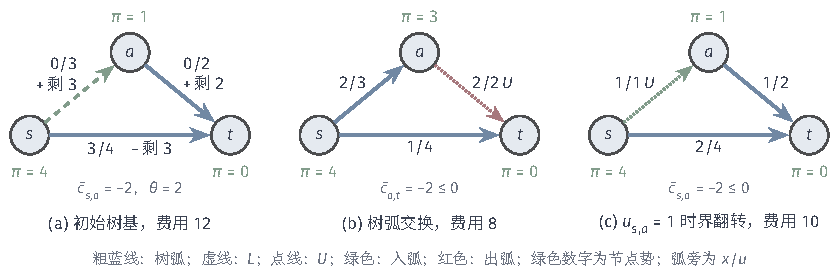
\includegraphics[width=142.053mm]{figures/01-basic-mathematics/04-graphs/tikz/c3-ns-pivots/figure.pdf}
  \caption{第二阶段的两种迭代。弧旁为流量/容量，“$\pm$剩”为沿基本环的剩余量。(a)$\bar c_{s,a}=-2$，最多推送$2$单位。(b)树弧$a\to t$出基进入$U$，费用$12\to8$。(c)$u_{s,a}=1$时入弧自身先到上界，树不变，费用$10$。}
  \label{fig:graph-opt-ns-pivots}
\end{figure*}

图~\ref{fig:graph-opt-ns-degenerate}在原网络上构造一次退化换基：把$s\to t$的容量改为$1$，从$T=\{s\to a,a\to t\}$、$U=\{s\to t\}$出发，流量$(2,2,1)$，树弧$a\to t$已在上界。以$t$为根，势为$(2,1,0)$，$s\to t$在上界而$\bar c_{s,t}=4-2+0=2>0$，应反向进入；基本环上$a\to t$要增加流量，剩余量为$0$，所以$\theta=0$。$a\to t$出树进入$U$，$s\to t$入树，流量和费用不变而树基变了；新势$(4,3,0)$下$\bar c_{a,t}=-2\leq0$，算法停止。这次退化换基换来了证书，一般情形下连续退化则可能循环。

\begin{figure}[!htb]
  \centering
  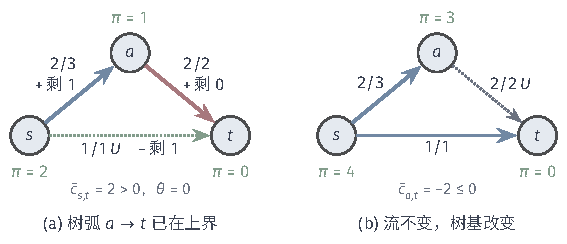
\includegraphics[width=96.054mm]{figures/01-basic-mathematics/04-graphs/tikz/c3-ns-degenerate/figure.pdf}
  \caption{退化换基（$u_{s,t}=1$）。(a)入弧$s\to t$（绿色）在上界且约化费用为正，反向进入；树弧$a\to t$（红色）剩余量为零，步长为零。(b)$a\to t$出基后流量与费用不变，新势满足最优性条件。}
  \label{fig:graph-opt-ns-degenerate}
\end{figure}

\subsubsection{正确性与复杂度}

三点改道可分三件事检查：仍送到$3$单位，不超容量，每单位费用降$2$。一般情形逐项对应：环上每个顶点一进一出，净流出不变；步长取环上剩余量的最小值，上下界仍满足；费用变化等于步长乘以入弧在调整方向上的负约化费用。表示也保持合法：树弧交换删去的出弧在基本环上，删去后树仍连通无环，新的$T$仍是生成树，出弧落在它到达的界上，被正确归入$L$或$U$；界翻转只改变入弧的界状态。

树流由树基唯一确定，这可以用关联矩阵说明。按第~\ref{sec:graph-representations}节的约定，关联矩阵$\bm B$中弧$(i,j)$对应的列在第$i$行为$1$、第$j$行为$-1$，守恒式就是$\bm B\bm x=\bm b$。$\bm B$各行之和为零，删去根所在的一行不丢失信息，记剩下的矩阵为$\tilde{\bm B}$，树弧对应的列组成$(n-1)$阶方阵$\tilde{\bm B}_T$。按消去叶子的次序排列行与列，每消去一个叶子，它所在的行在剩余树弧列中只有一个非零元，所以$\tilde{\bm B}_T$经重排后是对角元为$\pm1$的三角矩阵，从而可逆。于是$\bm x_T=\tilde{\bm B}_T^{-1}(\tilde{\bm b}-\tilde{\bm B}_N\bm x_N)$唯一确定，其中$N=L\cup U$。

\begin{theorem}[网络单纯形法的正确性]
\label{thm:graph-opt-network-simplex}
在精确运算下，采用词典序规则的网络单纯形法在有限轮后停止。第一阶段最优人工流为零当且仅当原问题可行；可行时第二阶段输出的流是最小费用流，停止时的势与之构成最优性证书。若供需与上下界都是整数，输出的流为整数流。
\end{theorem}

\begin{proof}
有限终止：在一个阶段内，扰动后的供需固定不变，扰动后的流由树基唯一确定，所以扰动后的费用是树基的函数。词典序规则使扰动后的问题保持非退化，每轮扰动后的步长严格为正，扰动后的费用严格下降（第~\ref{sec:graph-opt-ns-improvements}小节证明），因此已出现过的树基不会再出现。$T$是有限多棵生成树之一，每条非树弧只有两种界状态，树基只有有限个，所以每个阶段在有限轮后停止。

可行性判定：若原问题有可行流，配上全零人工流就是第一阶段的可行解，目标为零，所以最优值为零；反之，最优值为零时人工弧全部空载，原弧流量满足原问题的全部约束。最优性：每个阶段停止时树弧约化费用为零，非树弧满足所在界对应的符号条件，由定理~\ref{thm:graph-opt-potential-certificate}，当前流在本阶段的费用下最优。整数性：初始星形树的流量是供需本身；树流由三角方程组逐叶解出，每步只做整数加减；步长是若干个整数剩余量的最小值，沿环更新仍是整数加减。所以每轮的流都是整数流。
\end{proof}

整数性为第~\ref{sec:graph-opt-mcf-unified}小节的归约提供依据：只要可行，就存在整数最优流。第二阶段从清理后的树基重新设置扰动，有限终止的论证在两个阶段分别成立。

设顶点数为$n$，弧数为$a$。每轮扫描全部非树弧定价需要$O(a)$；沿父指针找基本环、比较剩余量、更新流量都是$O(n)$；沿新树重新求父顶点、深度与势也是$O(n)$。所以每轮主要操作为$O(n+a)$。流量、界与费用的数组占$O(a)$，树记录与势占$O(n)$；词典序规则另为每条树弧存储$n-1$个扰动系数，共$O(n^2)$，每轮比较和更新这些系数也需$O(n^2)$。总开销还取决于迭代轮数，其中包括退化换基；有限性论证只给出与树基个数相当的上界，不能从单轮开销推出统一的多项式总时间界。

\subsubsection{实现改进与数值处理}
\label{sec:graph-opt-ns-improvements}

词典序规则的完整构造作为补充阅读。把上界写成等式$x_{i,j}+s_{i,j}=u_{i,j}$，$s_{i,j}\geq0$是上界松弛量。每条弧有两个离界距离$x_{i,j}-\ell_{i,j}$与$s_{i,j}$；只有每条树弧的两个离界距离都为正，步长才一定为正。词典序规则用符号扰动人为地制造这种非退化情形。在一个阶段开始时，把当前可行树基的树弧编号为$e_1,\ldots,e_{n-1}$，把$e_k$的流量改为$x_{e_k}+\sigma_k\varepsilon^k$：若$e_k$在上界取$\sigma_k=-1$，否则取$\sigma_k=+1$。供需随之改为扰动后流量对应的净流出，并在整个阶段内保持不变；非树弧仍恰在界上。$\varepsilon$是充分小的正数，每个量记为$(\text{常数},\varepsilon\text{的系数},\ldots,\varepsilon^{n-1}\text{的系数})$，从常数项起逐分量比较，即词典序比较。这样每条树弧的两个离界距离在词典序下都严格为正。

每轮比较步长时，增加流量的树弧以$u-x(\varepsilon)$为候选，减少流量的树弧以$x(\varepsilon)-\ell$为候选，入弧以$(u-\ell,0,\ldots,0)$为候选，取词典序最小者作为步长$\theta(\varepsilon)$并让它出基，所有树弧的扰动流量按$\theta(\varepsilon)$一同更新。还原到基本环上，这个规则只在实际步长并列时起作用：比较并列阻塞弧的$\varepsilon$系数，选词典序最小者出基，实际流量仍按常数项更新。三点网络的第一阶段按$s\to r$、$r\to t$、$a\to r$的次序设置扰动，流量为$3-\varepsilon$、$3-\varepsilon^2$、$\varepsilon^3$；$s\to t$入树时$s\to r$与$r\to t$的候选向量为$(3,-1,0,0)$与$(3,0,-1,0)$，前者更小，所以$s\to r$出基。

\begin{proof}[词典序规则保持非退化的证明（补充阅读）]
初始时各树弧的$\varepsilon$系数行是$\pm$单位向量，线性无关。每次树弧交换，留下的树弧系数行加减出弧的系数行，入弧取出弧系数行的正负，这是可逆的行变换；界翻转不改变系数行。所以树弧的系数行始终线性无关，两条树弧的候选向量不会相等，入弧的候选向量只有常数项，也不会与树弧的相等，词典序最小者唯一。更新后出弧恰好落在界上，其余树弧仍在词典序下严格离界，扰动后的问题始终非退化，每轮的$\theta(\varepsilon)$在词典序下严格为正。扰动后的费用改变量为$\theta(\varepsilon)$乘以负的约化费用，因而严格下降。
\end{proof}

另一类常用规则维护所谓强可行树，有自己的方向约定与初始化要求；第一阶段清理只得到普通的可行树基，两类规则不能混用。

常见的实现改进只改变维护代价，不改变可行性与最优性条件。一是局部更新势：删去出弧后树分成两块，只有不含根的一块的势同加或同减入弧的约化费用，只需遍历这棵子树。二是按先序后继与子树大小存储树，换基时只重排被移动的子树。三是分块定价：每轮只扫描一部分非树弧，找到违反条件的弧就入树。找环、界翻转和子树更新的写法可以对照NetworkX库中的网络单纯形实现\scite{math-graph-networkx-network-simplex}，但它的初始化与防循环规则另有前提，不能与本节的两阶段词典序版本混用。

精确整数数据下，上述判断都能精确进行。浮点实现中，守恒、弧界、约化费用的符号与步长比较都只能在容差内判断，例如把绝对值小于容差的约化费用当作零；容差过小会因舍入反复选弧，过大会漏掉改进方向。有限容量的主线不会出现费用无界。若扩展到无穷容量，还须处理增加方向剩余量全为无穷的基本环：这时步长无穷而入弧约化费用为负，存在可以无限推送的负费用环，应报告费用无下界。

\subsection{最大流、匹配与指派的统一表示}
\label{sec:graph-opt-mcf-unified}

前面三节的问题都能写成最小费用流。最大流的流值不固定，不能直接写成供需，办法是令全部$b_i=0$，原弧费用为零，再加一条从$t$回到$s$的回边，容量取源点原出弧容量之和，费用为$-1$。对任一循环流，由源点守恒，$s$经原弧的净流出等于回边流量$x_{t,s}$，即原网络的源汇流值，总费用为它的相反数。反过来，值为$v$的流配上$x_{t,s}=v$就是循环流，$v$不超过源点出容量，回边容量够用。于是最小费用循环流对应最大流，最小费用就是负的最大流值。只设零费用而不加回边则不够：全零流已是最优。

二部最大匹配沿用第~\ref{sec:graph-opt-match-alternating}小节的单位容量网络：$s$连向左侧各顶点，允许边从左指向右，右侧各顶点连向$t$，容量都是$1$、费用为零，再加入上述费用为$-1$的回边，容量取两侧顶点数的较小者。由定理~\ref{thm:graph-opt-network-simplex}的整数性，存在整数最优循环流，其中间弧上流量为$1$的弧两两不共享端点，构成匹配，配对数等于回边流量；反之每个匹配都给出这样的循环流，所以费用最小等同于配对数最多。

$r$阶指派在同一个单位容量配对网络中固定输送量$r$：令$b_s=r$、$b_t=-r$，中间弧的费用为配对成本$c_{i,j}$，其余弧费用为零，不加回边。整数可行流使每个左侧顶点恰送出一单位、每个右侧顶点恰收到一单位，对应一个完美匹配，总费用就是指派成本。由整数性，只要可行就存在整数最优流，它给出最优指派；若送不出$r$单位，说明不存在完美匹配，指派不可行。若要最大化收益，费用取收益的相反数；矩形问题按第~\ref{sec:graph-opt-assign-rectangular}小节补成方阵后写入网络，求解后删去虚拟配对。

图~\ref{fig:graph-opt-problem-relations}汇总了这些关系。最小费用流保留了一般的容量与供需；最大匹配只求配对数量，指派在完整配对的条件下比较成本。专门算法利用各自的结构：最大流算法只沿源汇方向增广，匈牙利算法与Hopcroft--Karp算法只记录配对伙伴，KM算法的标号与Auction算法的价格是二部图上的节点势。统一表示说明问题可以转化，并不意味着网络单纯形法在所有输入上都优于专门算法。

\begin{figure}[!htb]
  \centering
  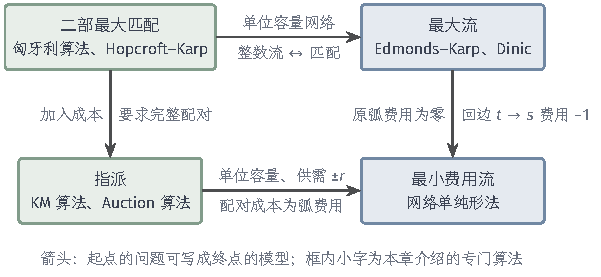
\includegraphics[width=101.829mm]{figures/01-basic-mathematics/04-graphs/tikz/c3-problem-relations/figure.pdf}
  \caption{本章四种流与配对问题之间的模型关系。箭头表示起点的问题可以写成终点的模型：二部最大匹配是单位容量的最大流，加入成本并要求完整配对就成为指派；最大流加入费用为$-1$的回边后成为最小费用循环流；指派是供需为$\pm r$的单位容量最小费用流。框内小字是本章介绍的专门算法。}
  \label{fig:graph-opt-problem-relations}
\end{figure}

\subsection{结果检验}
\label{sec:graph-opt-ns-analysis}

输出须回到原始问题检查。先把下界平移量加回流量，核对每个顶点的净流出等于原始$b_i$、每条弧满足原始上下界；再按原始费用重算目标值，确认它等于平移后问题的费用加上常数$\bm c^{\top}\bm\ell$。最优性则用输出的势逐弧核对条件~\eqref{eq:graph-opt-mcf-certificate}。可行性与最优性分别验收：前者只看流，后者还要看势。浮点结果应分别报告守恒、弧界与约化费用符号的误差；在容差内近似满足的条件不能当作精确证书。

回看第~\ref{sec:graph-max-flow}节到本节，四类问题共用几个认识：残量方向允许撤回旧选择；二部配对的结构简化了搜索；引入成本后，第~\ref{sec:graph-opt-assign-labels}小节的可行标号与第~\ref{sec:graph-opt-auction}小节的价格为成本提供可核查的界；一般网络再用节点势和沿环调整优化，节点势正是标号与价格的推广。章末据此比较各类证书与输入条件。
